\documentclass{jsarticle}

\usepackage[dvipdfmx]{graphicx}
\usepackage{float} %図を指定の位置に置
\usepackage{moreverb}

\begin{document}
 
\begin{center}
\vspace*{1cm}
\large
{\LARGE 卒業研究報告書}\\
\vspace*{0.8cm}
題目\\
\vspace*{1cm}
{\Huge \underline{プロセスマイニングを用いた} \\ \underline{店舗に並ぶ行列の分析}}
\vspace{3mm}
 
\vspace*{3cm}
指導教員\\
\vspace*{0.3cm}
\underline{\LARGE 森山 真光 准教授}\\
%\vspace*{-0.3cm}
%\underline{\hspace*{5cm}}\\
\vspace*{3cm}
報告者\\
\vspace*{0.3cm}
 
{19--1--037--0177}\\
\vspace*{0.3cm}
\underline{\Huge 李 晃史}\\
% \vspace*{-0.3cm}
% \underline{\hspace*{5cm}}\\
\vspace*{0.5cm}
近畿大学理工学部情報学科\\
\vspace*{2cm}
提出日:\today 
\end{center}
 
\newpage
\normalsize

%\maketitle
\tableofcontents



\newpage

\section{序論}
\subsection{本研究の背景}
近年、コロナ禍により飲食店におけるテイクアウトの需要が高まっている。
飲食店においてテイクアウトの需要が高まっている事を示すデータがいくつかある。
株式会社プレシャスパートナーズが行なった931の飲食店から得た年末の営業に関しての
調査\cite{bibi6}では、テイクアウトを行なっていると回答したのが68.5\%、
その中で新型コロナウイルスの影響でテイクアウトを始めたと回答したのが54.7\%と半数以上になる。
また日本政策金融公庫による飲食店のテイクアウト・デリバリーサービス等に関する
消費者調査結果\cite{bibi7}では、コロナ禍が収束してからもテイクアウトを利用したいと考えている人が
多いことから、コロナ禍の状況に関わらずこれからも拡大していくものだと考えられる。

そんな中、店舗販売と併用してモバイルオーダーでのテイクアウト注文を導入した店舗で、
モバイルオーダーでのテイクアウト注文を無制限に受け入れ過ぎたことによって店舗が混雑し
販売に支障をきたす事態[1]や、逆に注文の受け入れ制限をしたことにより早く注文を処理できた場合に
本来受け入れることができた注文分の利益を損失する事態が起きている。
従ってモバイルオーダーでのテイクアウト注文を無制限に受け入れるのではなく、
利用率がある一定の値を越えないように注文の受け入れ制限をすることで、
店舗での混雑による支障や利益損失を防ぐことができるのではないかと考えられる。

\begin{figure}[H]
  \centering
  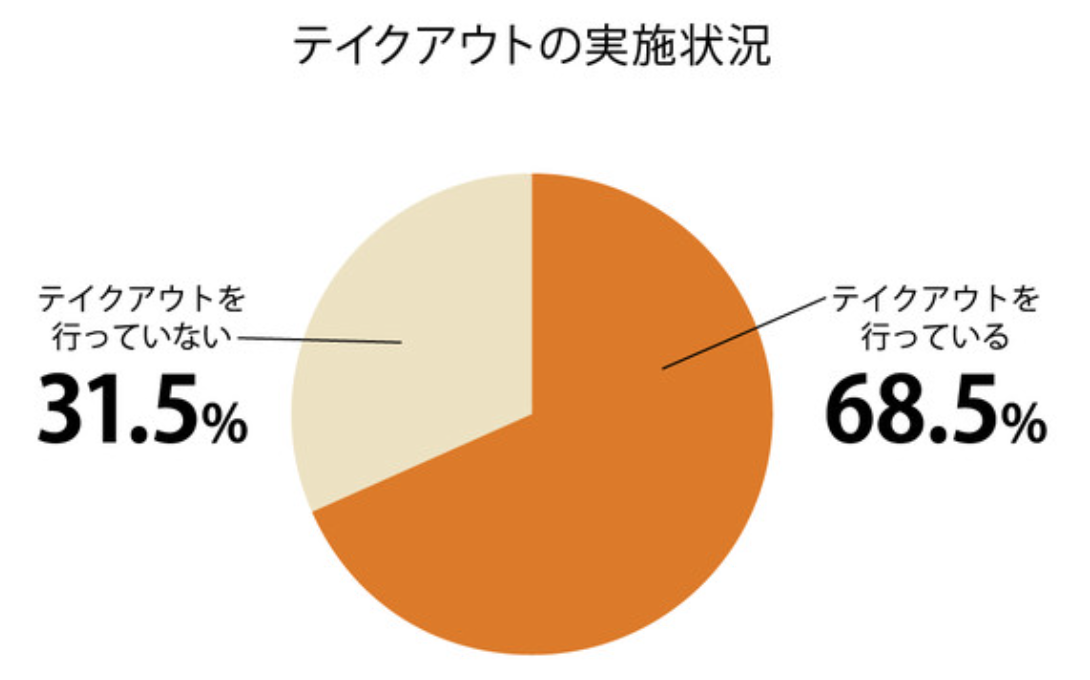
\includegraphics[width=7cm]{1.png}
  \caption{テイクアウトの実施状況}
  \scriptsize(出典:931の飲食店から得た年末の営業に関しての調査.株式会社プレシャスパートナーズ.)
  \label{fig:1}
\end{figure}

\begin{figure}[H]
  \centering
  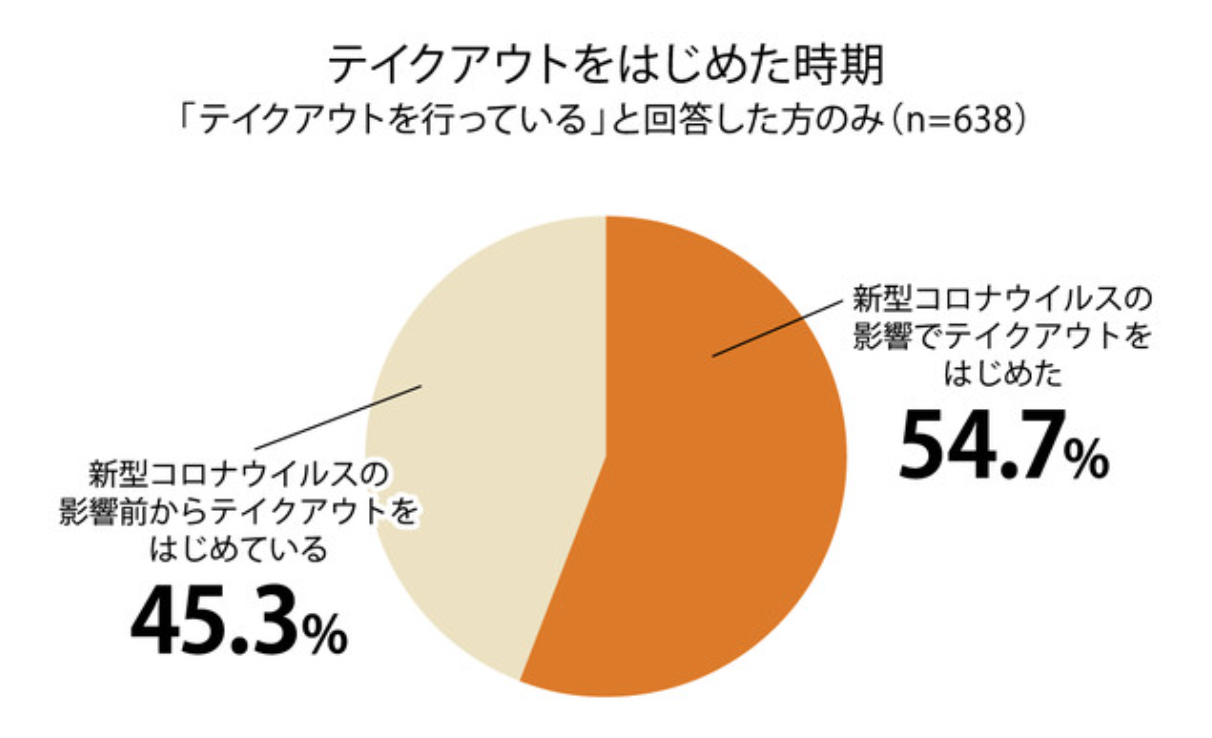
\includegraphics[width=7cm]{2.png}
  \caption{テイクアウトを始めた時期}
  \scriptsize(出典:931の飲食店から得た年末の営業に関しての調査.株式会社プレシャスパートナーズ.)
  \label{fig:2}
\end{figure}




\newpage

\subsection{本研究の目的}
店舗販売と併用してモバイルオーダーでのテイクアウト注文の受け入れ人数を無制限や適当に設定すると、店舗の混雑や利益損失を起こす可能性がある。

本研究では、適切な受け入れ人数を設定するために必要な行列分析を目的とし、
店舗の行列の計測を行いプロセスマイニングを用いて行列の分析を行う。
店舗での行列計測については、近畿大学東大阪キャンパスにある近大をすすらんか様に承諾を得て行った。



\subsection{本報告書の構成}
2章では関連技術と関連研究を示す。3章では

行列の計測を調べ、行列計測の効率化を測る




\newpage


\section{関連技術・研究}
\subsection{プロセスマイニング}
プロセスマイニングとは、従業員が操作する各種業務システムのイベントログに基づく
ビジネスプロセスを分析することで業務プロセスを自動的に可視化し、
問題箇所を特定する分析手法である。プロセス管理の分野における一連の技術である。
プロセスマイニングは、大企業などで商品購入までのプロセス改善などに導入されている。
記録されたイベントログに含まれる傾向、パターン等の詳細を識別するために
イベントログに特殊なデータマイニングアルゴリズムを適用する。
プロセスマイニングを用いた分析からは除去しても支障のない「無駄な業務」や、
処理待ちが発生しやすくイベント全体の時間を長引かせてしまっている
「ボトルネック」などの問題を発見できる。
また、各イベントを行うのにかかった時間や平均時間を抽出し、
一定の時間間隔でのデータやグラフを得ることができる。

本研究では、プロセスマイニングのツールとしてApromoreを使用する。
図\ref{fig:3}にApromoreの分析画面を示す。

\begin{figure}[H]
  \centering
  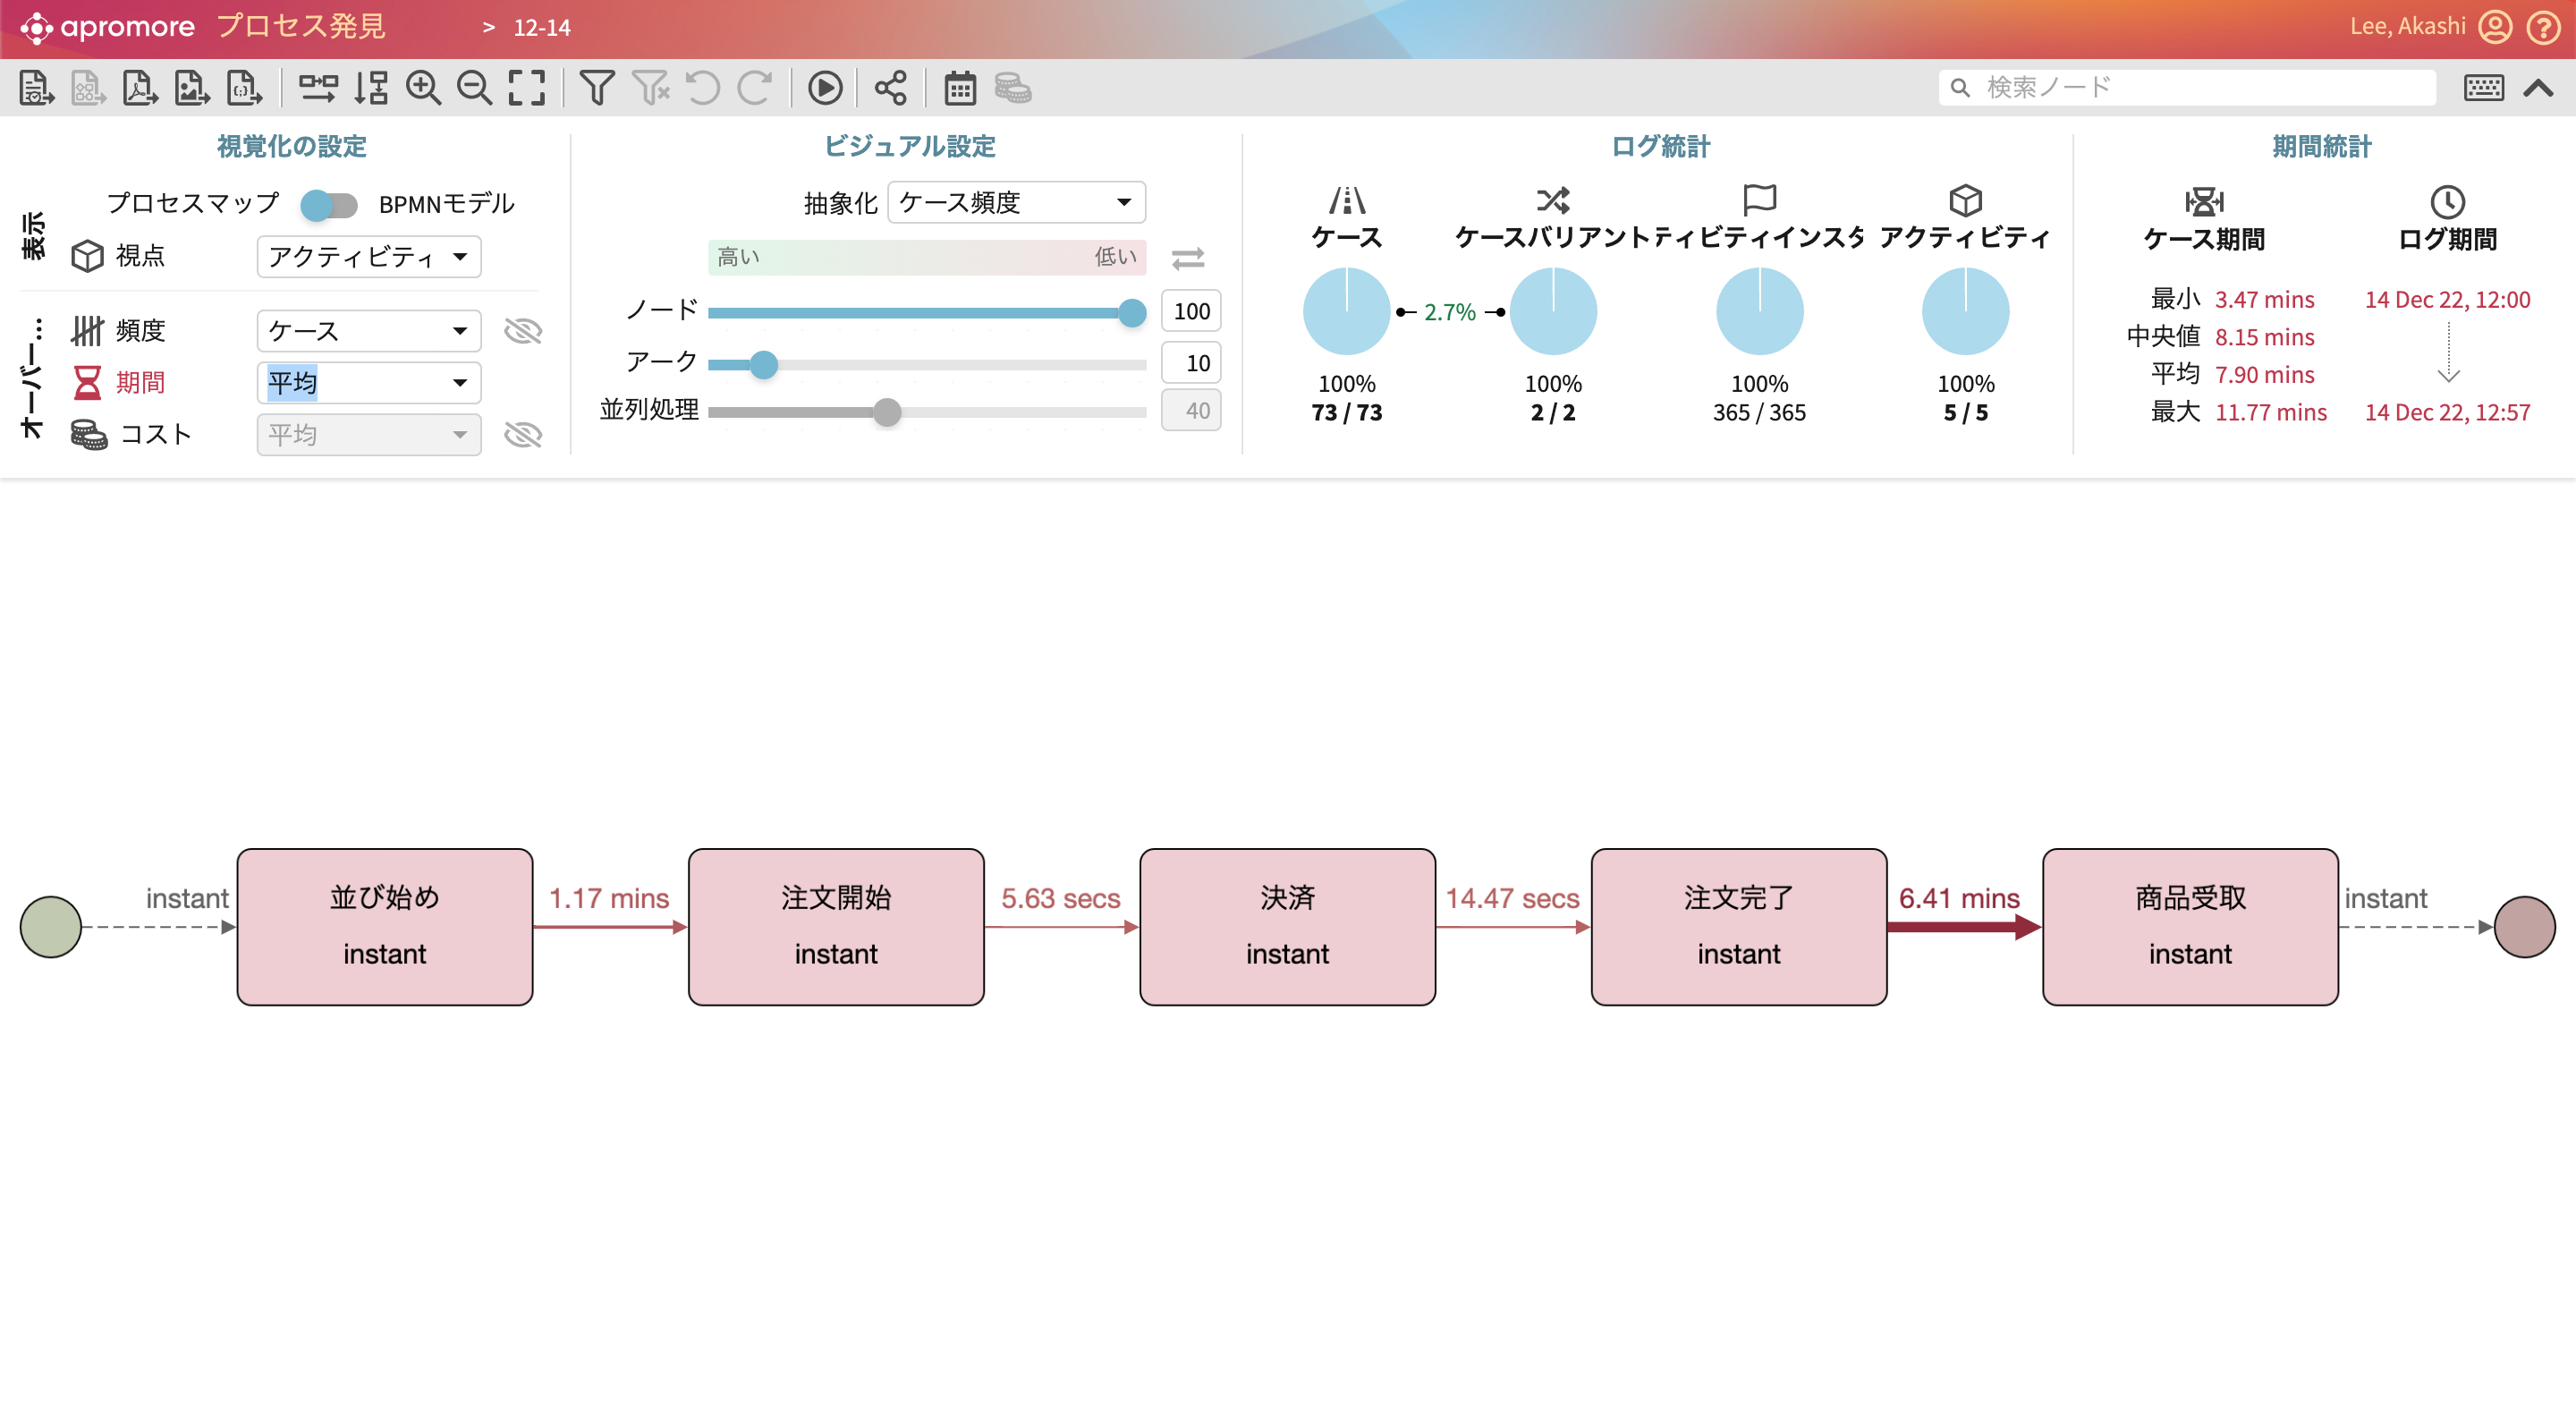
\includegraphics[width=15cm]{3.png}
  \caption{Apromoreの分析画面}
  \label{fig:3}
\end{figure}



\newpage

\subsection{関連研究}

店舗における行列を分析するために飲食店の形態を把握することやレジや受け取り口での
スタッフの人数の変更による影響などを参考にした。
こちらでは注文会計を済ませ商品を受け取るまでの待ち時間は、
顧客満足度に影響がある\cite{bibi8}と述べている。
そのためスマートフォンなどでの事前注文決済を行うことで注文決済の待ち時間をゼロにすることは
非常に有効であるがそれと半面に店舗が混雑しキャパオーバーを起こす状況\cite{bibi2}が
あると指摘している。ここではモバイルオーダーを導入した店舗形態の評価を行うために様々な
パターンのモデルについて比較評価を行なっている。表\ref{table1}にパターンとその説明を示す。

\begin{table}[H]
 \begin{center}
   \caption{店舗形態のパターン}
  \begin{tabular}{|c|l|} \hline
1-1     & レジ1人、商品提供1人\\ \hline
2-1     & レジ2人、商品提供1人\\ \hline
2-1(IT) & レジ1人とITによるレジ、商品提供1人\\ \hline
  \end{tabular}
 \label{table1}
 \end{center}
\end{table}

ここではモバイルオーダーを1人のレジスタッフのような扱いをしており、モバイルオーダーで注文を
した利用客は来店するとレジへ行かずにそのまま受け取り口へ向かい商品の受け取り待ちをする。
またレジでレジスタッフが商品提供スタッフのところに利用客を流さずに
そのまま自分で商品も準備して処理をするということも想定している。
これによりサービス時間が短くなる傾向があることに触れており、論文では考察されていないが
これは作業を並行して行うことによるサービス時間の減少であると考えられる。
また、シミュレーションでは行列の人数が増えるほど混雑を嫌って並ばなくなる人が増えることや、
モバイルオーダーの導入によりレジでの混雑が減ったことにより、
混雑を避けていた利用客が利用することによる利用率の向上にも配慮が必要である。





\newpage

\section{研究内容}

\subsection{行列データの収集方法}
実店舗での行列計測については、近畿大学東大阪キャンパスにある近大をすすらんか(以下近大ラーメン)に承諾を得て行った。
近大ラーメン店では、レジの代わりに券売機を設置して食券を購入し半券を渡すと注文が通る仕組みとなっている。
近大ラーメンの利用者は、来店して列がない場合は待ち時間なしですぐに券売機にて食券を購入する。列があれば並び先頭になった際に券売機にて食券を購入し、
半券を渡し注文が終了すると待ちの行列に移動する。
ここでは具体的に列に並ぶわけではないが基本的に注文順に商品は受け渡される。
商品の準備が終了すると商品を確認して受け取り、受け取り待ちの行列から抜ける。
行列から取得したいタイムスタンプは、行列参加時間,注文開始時間,決済開始時間,注文完了時間,商品受け取り時間の5つである。さらに男女の区分やグループ毎の人数の区分のデータも取得する。
表\ref{table2}に近大ラーメンにおける店舗フローと取得するタイムスタンプの対応表を示す。

\begin{table}[H]
 \begin{center}
   \caption{近大ラーメンにおける店舗フローと取得するタイムスタンプの対応表}
   \begin{tabular}{|c|c|} \hline
店舗フロー      & タイムスタンプ \\ \hline \hline
列があれば並ぶ   & 行列参加時間 \\ \hline
券売機の先頭     & 注文開始時間 \\ \hline
券売機にお金投入  & 決済開始時間 \\ \hline
半券を渡す       & 注文完了時間 \\ \hline
料理を受け取る   & 商品受け取り時間 \\ \hline
  \end{tabular}
 \label{table2}
 \end{center}
\end{table}

行列の計測方法は、行列計測用のアプリケーション(以下ExpoGo)\cite{bibi4}を用いて行う。
ExpoGOのUIを図\ref{fig:4}に示す。


\begin{figure}[H]
  \centering
  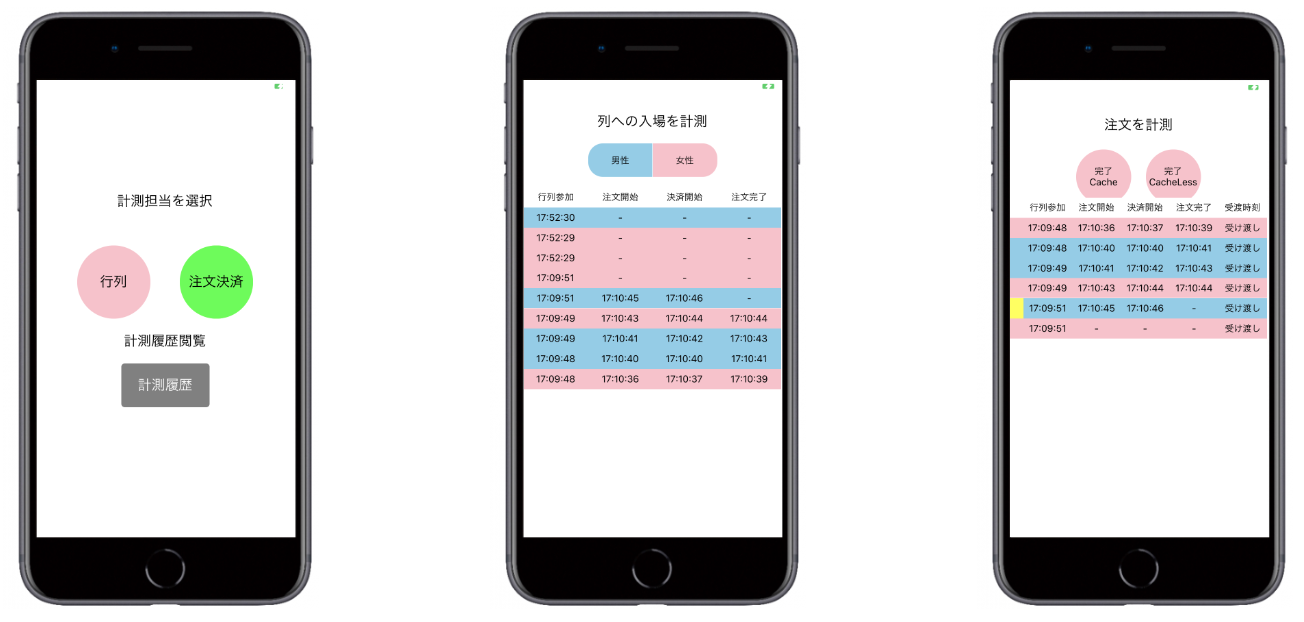
\includegraphics[width=14.5cm]{4.png}
  \caption{ExpoGO(左からホーム画面、行列参加、注文決済)}
\scriptsize(出典:事前注文・事前決済プラットフォームの開発と導入による待ち行列の評価-事前注文・事前決済プラットフォームの開発.藤井遼.)
  \label{fig:4}
\end{figure}


図\ref{fig:4}の一番左の画面は行列計測のホーム画面であり、
ピンク色の丸で囲まれた「行列」を押下すると真ん中の行列参加計測画面に遷移し、
緑色の丸で囲まれた「注文決済」を押下すると一番右の注文決済計測画面に遷移する。
複数台のデバイスからでもリアルタイムに計測が可能となっているため、
行列の計測は3人以上が望ましいが、2人でも問題なく計測可能となっている。
2人の役割分担は、一人は行列参加者を計測し何人で来たのかをメモする。
もう一人は、注文開始時間、決済開始時間、注文完了時間、受け渡し時間を計測する。


取得するタイムスタンプのデータとデータキーの一覧を表\ref{table3}に示す。
また、集合Tの各差分を求める事で行列時間、注文時間、決済時間、受け取り待ち時間を算出できるので
表\ref{table4}に差分関係を示す。



\begin{table}[H]
 \begin{center}
   \caption{取得するタイムスタンプのデータとデータキーの一覧}
   \begin{tabular}{|c|l|l|l|} \hline
ti & データキー     & 取得データ      & データ例 \\ \hline \hline
t1 & queueing\_at  & 行列参加時間    & 2022-07-21 10:00:00 \\ \hline
t2 & ordered\_at   & 注文開始時間    & 2022-07-21 10:01:00 \\ \hline
t3 & paymented\_at & 決済開始時間    & 2022-07-21 10:02:00 \\ \hline
t4 & serviced\_at  & 注文完了時間    & 2022-07-21 10:03:00 \\ \hline
t5 & handed\_at    & 商品受け取り時間 & 2022-07-21 10:05:00 \\ \hline
  \end{tabular}
 \label{table3}
 \end{center}
\end{table}



\begin{table}[H]
 \begin{center}
   \caption{算出する項目と差分関係}
   \begin{tabular}{|c|c|} \hline
算出する項目 & 差分関係 \\ \hline \hline
行列時間 & $t2-t1$ \\ \hline
注文時間 & $t3-t2$ \\ \hline
決済時間 & $t4-t3$ \\ \hline
受取時間 & $t5-t4$ \\ \hline
  \end{tabular}
 \label{table4}
 \end{center}
\end{table}




\subsection{データの分析計画}
取得したイベントログのデータをCSVファルに変換し、Apromoreを使用してプロセスマイニングを行う。
プロセスマイニングでプロセスを可視化するために最低限必要となるイベントログのデータ項目は、
一連の作業をひも付ける「ケースID」、各活動を示す「アクティビティ」、
活動が実行された日時の「タイムスタンプ」の3つである。そのほかにも自由に追加することができる。
今回の計測では、行列参加時間、注文開始時間、決済開始時間、注文完了時間、商品受け取り時間の5つの区分に加えて男女の区分やグループ毎の人数の区分のデータも取得するので、
グループ人数と性別の項目を追加してデータを取得しCSVファイルを作成した。

CSVファイルに変換したデータをプロセスマイニングを用いて分析すると行列時間、注文時間、
決済時間、受取時間などの平均時間を求めることができる。
またフィルタリングを行い、注文する際の男女間での差や、グループ間での人数の違いによって生じる時間を分析する。




\newpage

\section{結果・考察}

\subsection{プロセスマイニングを用いた行列データの分析}
近大ラーメンで計測した日時と計測した項目の一覧を表\ref{table5}に示す。
7月の行列計測は行列参加時、注文開始時、決済開始時、注文完了時、商品受取時の5つの区分に分けて計測した。
12月の行列計測は7月に計測した上記の5つの区分に加えて、
新たに男女の項目とグループ人数の項目も追加して計測を行った。

\begin{table}[H]
 \begin{center}
   \caption{計測日程と計測項目}
   \begin{tabular}{|c|c|c|c|c|c|c|c|} \hline
日時 & 行列参加 & 注文開始 & 決済開始 & 注文完了 & 商品受取 & グループ人数 & 性別 \\ \hline \hline
2022/07/08 12:00〜13:00 & ○ & ◯ & ◯ & ◯ & ◯ & × & × \\ \hline
2022/07/11 12:00〜13:00 & ○ & ◯ & ◯ & ◯ & ◯ & × & × \\ \hline
2022/07/12 12:00〜13:00 & ○ & ◯ & ◯ & ◯ & ◯ & × & × \\ \hline
2022/12/14 12:00〜13:00 & ○ & ◯ & ◯ & ◯ & ◯ & ◯ & ◯ \\ \hline
2022/12/16 12:00〜13:00 & ○ & ◯ & ◯ & ◯ & ◯ & ◯ & ◯ \\ \hline
  \end{tabular}
 \label{table5}
 \end{center}
\end{table}




\subsubsection{計測結果}

%------------------------------------------------------------------
7月,12月に計測したデータを
図\ref{fig:708},図\ref{fig:711},図\ref{fig:712},図\ref{fig:1214},図\ref{fig:1216}に示す。
図\ref{fig:708}〜図\ref{fig:1216}は12:00〜13:00に計測したデータのプロセスマップであり、左から順に行列に並んだ時間、注文にかかった時間、決済から注文完了にかかった時間、
商品の受取待ち時間の各平均時間を表している。

\begin{figure}[H]
  \centering
  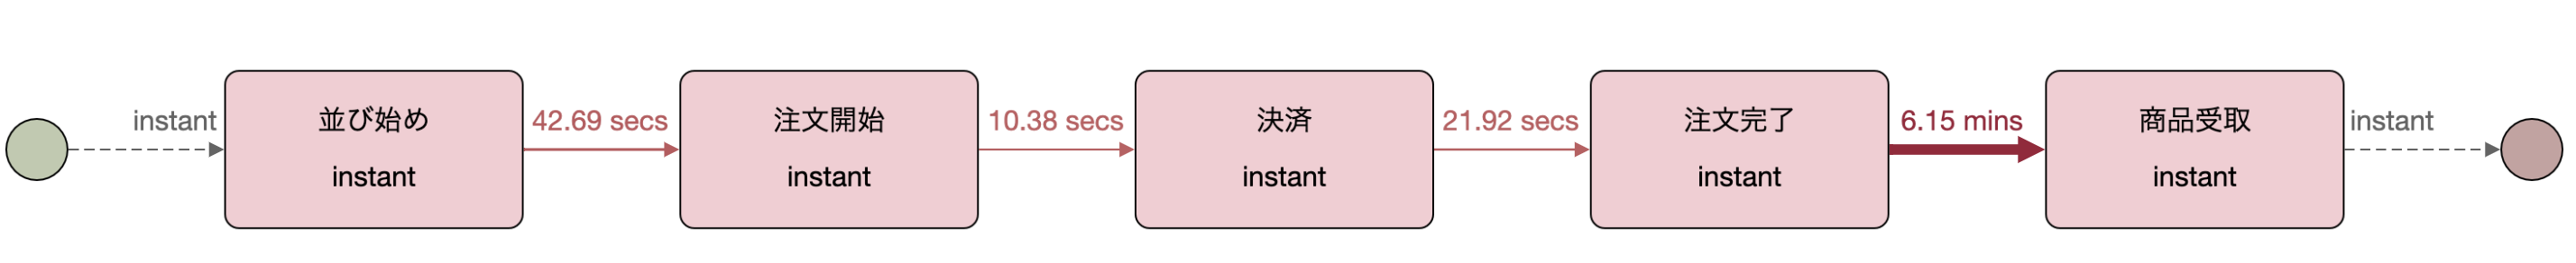
\includegraphics[width=15cm]{708.png}
  \caption{計測日時:7/8 12:00〜13:00,来店数:52人の各計測項目の平均時間}
  \label{fig:708}
\end{figure}

\begin{figure}[H]
  \centering
  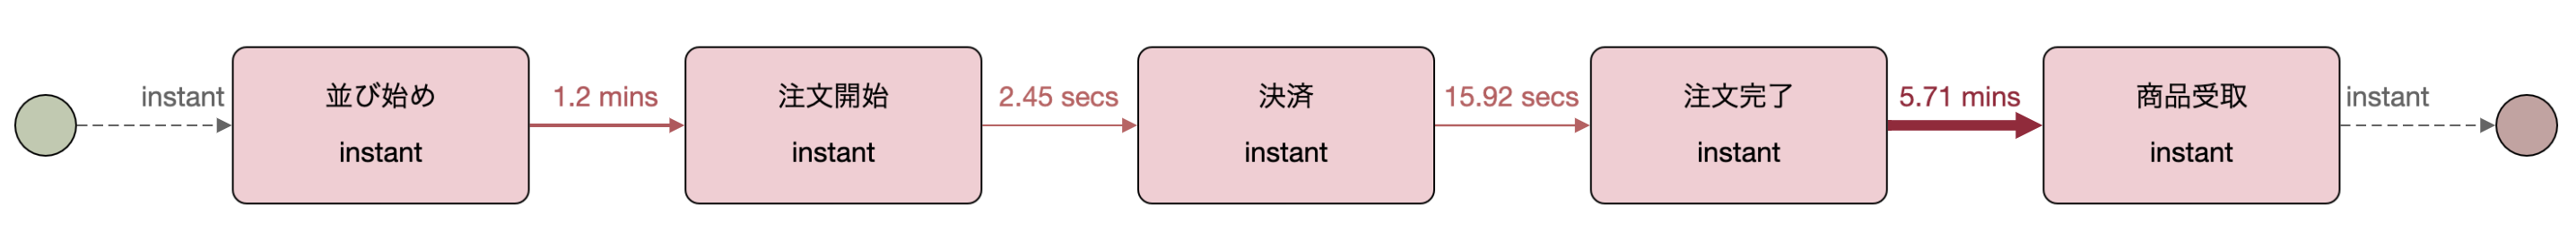
\includegraphics[width=15cm]{711.png}
  \caption{計測日時:7/11 12:00〜13:00,来店数:49人の各計測項目の平均時間}
  \label{fig:711}
\end{figure}

\begin{figure}[H]
  \centering
  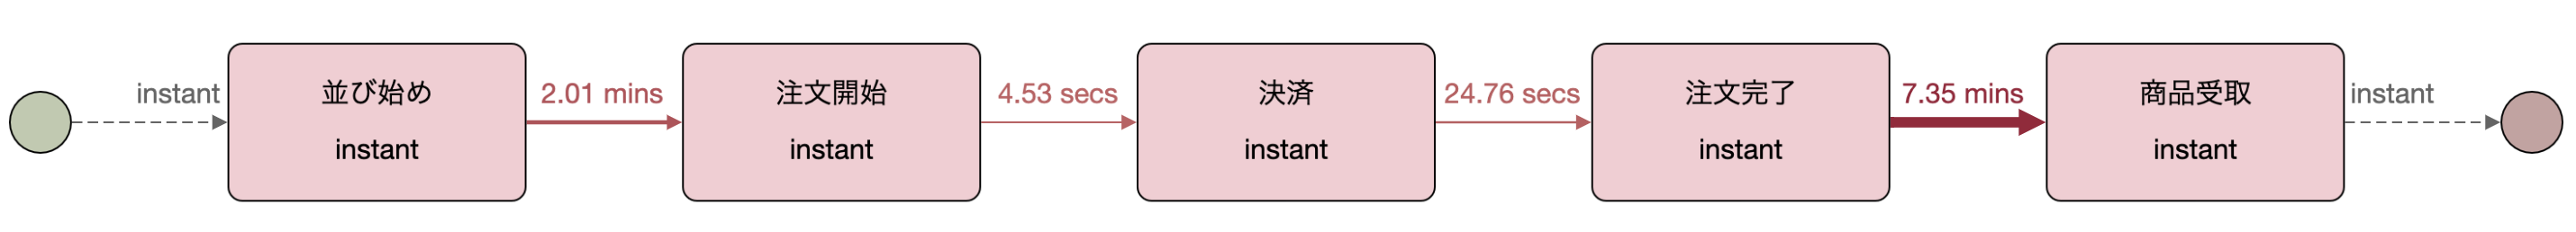
\includegraphics[width=15cm]{712.png}
  \caption{計測日時:7/12 12:00〜13:00,来店数:75人の各計測項目の平均時間}
  \label{fig:712}
\end{figure}

\begin{figure}[H]
  \centering
  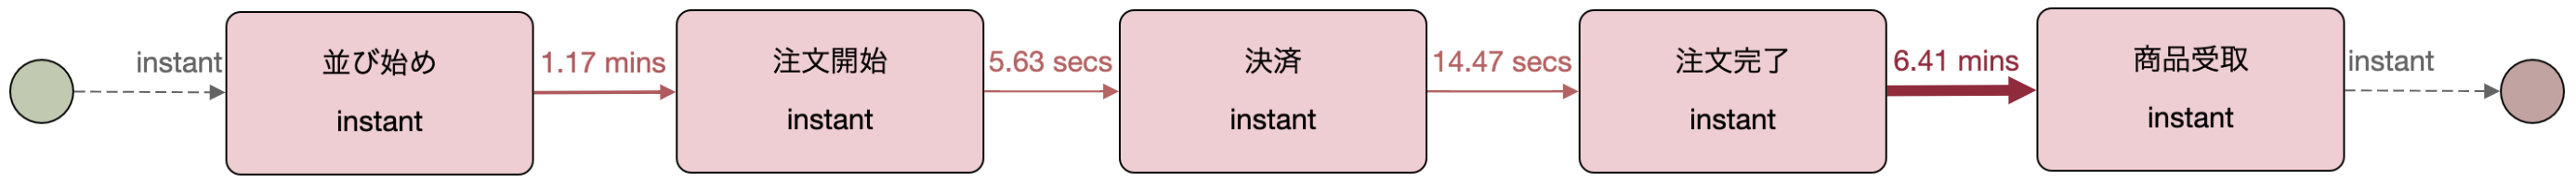
\includegraphics[width=15cm]{1214.png}
  \caption{計測日時:12/14 12:00〜13:00,来店数:73人の各計測項目の平均時間}
  \label{fig:1214}
\end{figure}

\begin{figure}[H]
  \centering
  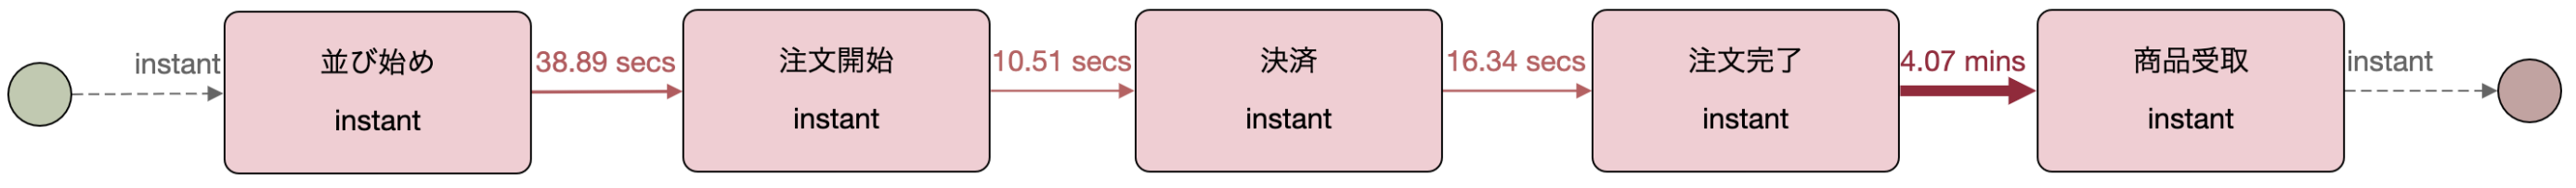
\includegraphics[width=15cm]{1216.png}
  \caption{計測日時:12/16 12:00〜13:00,来店数:61人の各計測項目の平均時間}
  \label{fig:1216}
\end{figure}
%------------------------------------------------------------------





%------------------------------------------------------------------
5日間を通して混雑したと思われる12:15〜12:30の時間軸の図と各計測項目の平均時間を示す。
\begin{itemize}
\item 7/8 12:15〜12:30のデータを図\ref{fig:708a},図\ref{fig:708b}
\item 7/11 12:15〜12:30のデータを図\ref{fig:711a},図\ref{fig:711b}
\item 7/12 12:15〜12:30のデータを図\ref{fig:712a},図\ref{fig:712b}
\item 12/14 12:15〜12:30のデータを図\ref{fig:1214a},図\ref{fig:1214b}
\item 12/16 12:15〜12:30のデータを図\ref{fig:1216a},図\ref{fig:1216b}
\end{itemize}

図\ref{fig:708a},図\ref{fig:711a},図\ref{fig:712a},図\ref{fig:1214a},
図\ref{fig:1216a}は12:15〜12:30以外のイベントログデータをフィルタリングしているのを表している。
図\ref{fig:708b},図\ref{fig:711b},図\ref{fig:712b},図\ref{fig:1214b},
図\ref{fig:1216b}は12:15〜12:30のデータのプロセスマップであり、
左から順に行列に並んだ時間、注文にかかった時間、決済から注文完了にかかった時間、
商品の受取待ち時間の各平均時間を表している。

\begin{figure}[H]
  \centering
  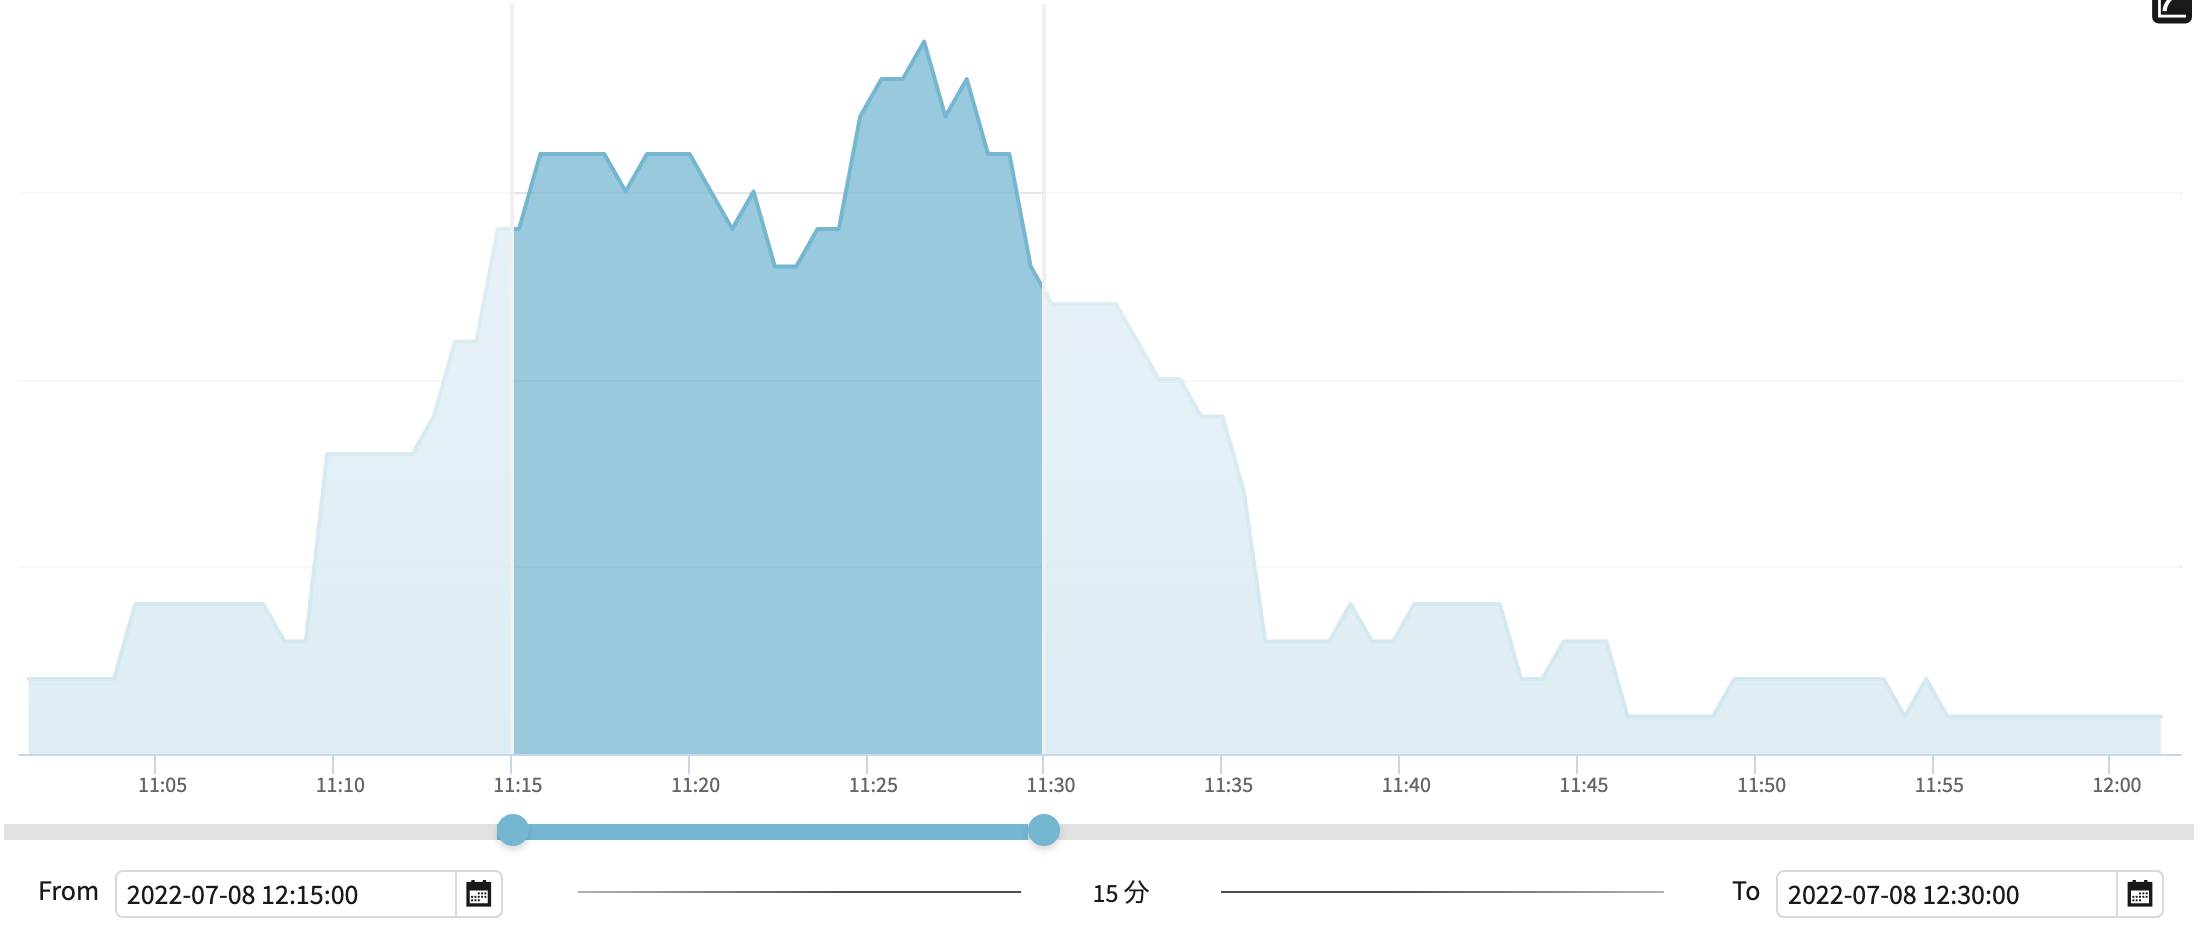
\includegraphics[width=14cm]{708a.png}
  \caption{計測日時:7/8 12:15〜12:30,来店数:37人の時間軸}
  \label{fig:708a}
\end{figure}

\begin{figure}[H]
  \centering
  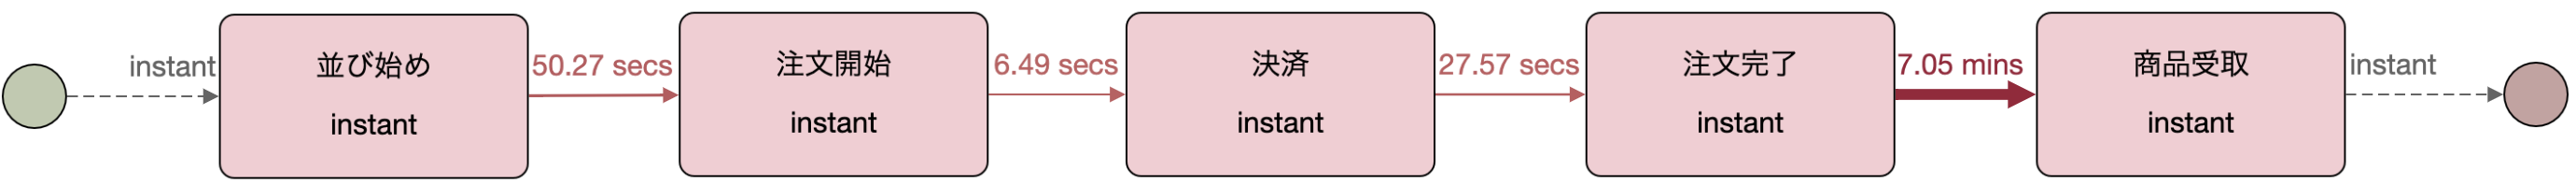
\includegraphics[width=15cm]{708b.png}
  \caption{計測日時:7/8 12:15〜12:30,来店数:37人の各計測項目の平均時間}
  \label{fig:708b}
\end{figure}


\begin{figure}[H]
  \centering
  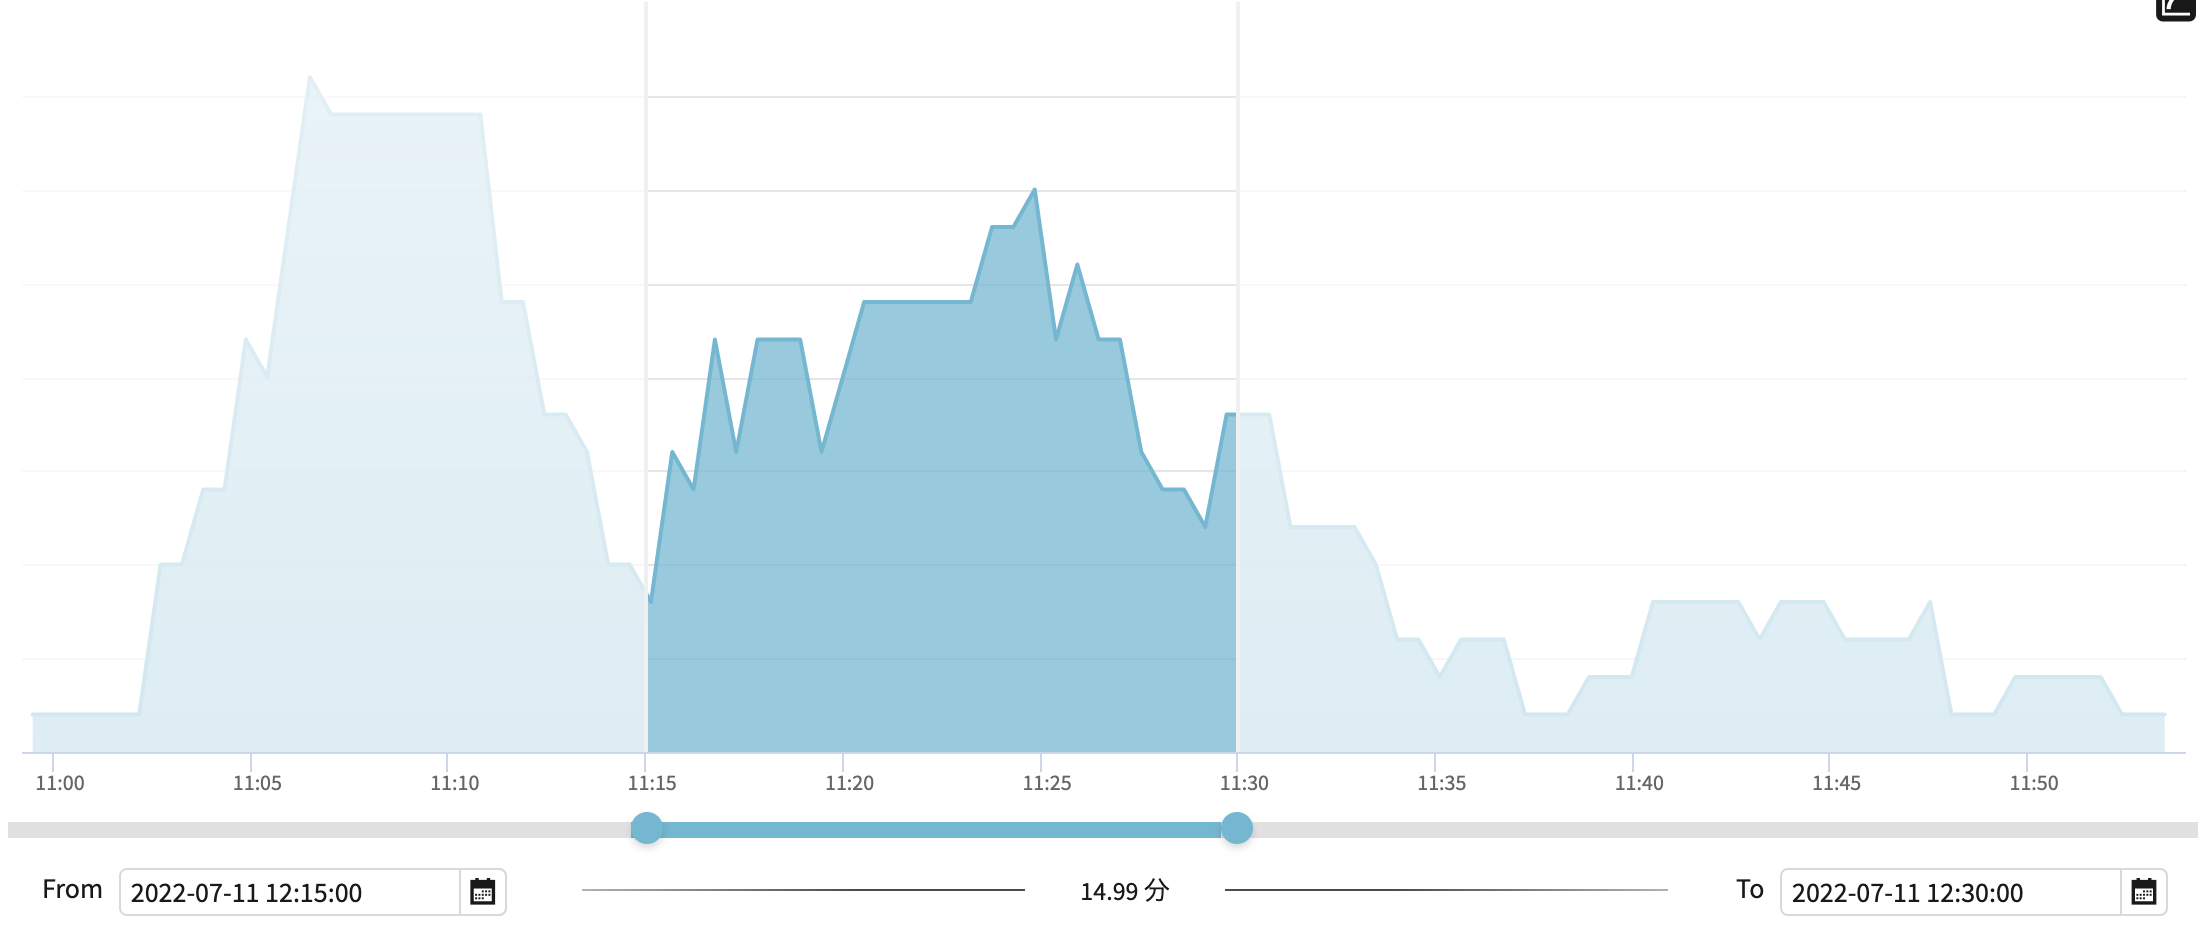
\includegraphics[width=14cm]{711a.png}
  \caption{計測日時:7/11 12:15〜12:30,来店数:27人の時間軸}
  \label{fig:711a}
\end{figure}

\begin{figure}[H]
  \centering
  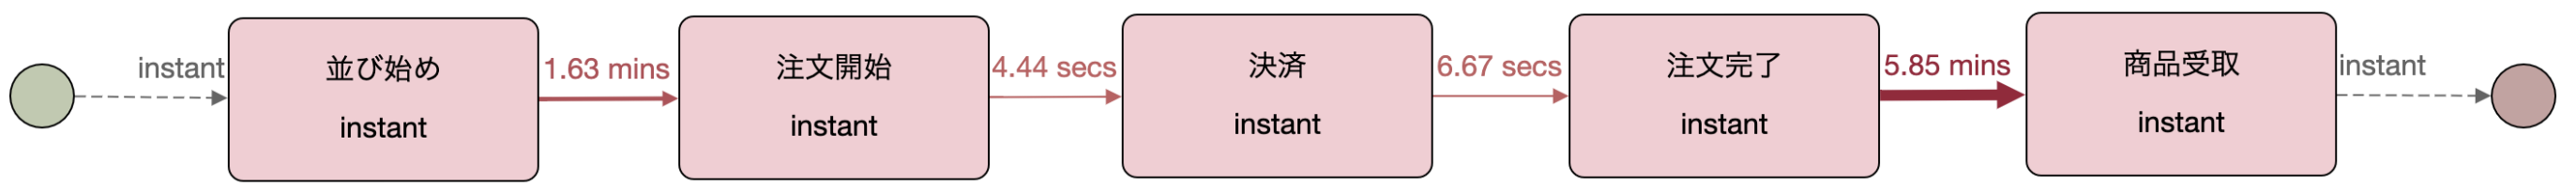
\includegraphics[width=15cm]{711b.png}
  \caption{計測日時:7/11 12:15〜12:30,来店数:27人の各計測項目の平均時間}
  \label{fig:711b}
\end{figure}


\begin{figure}[H]
  \centering
  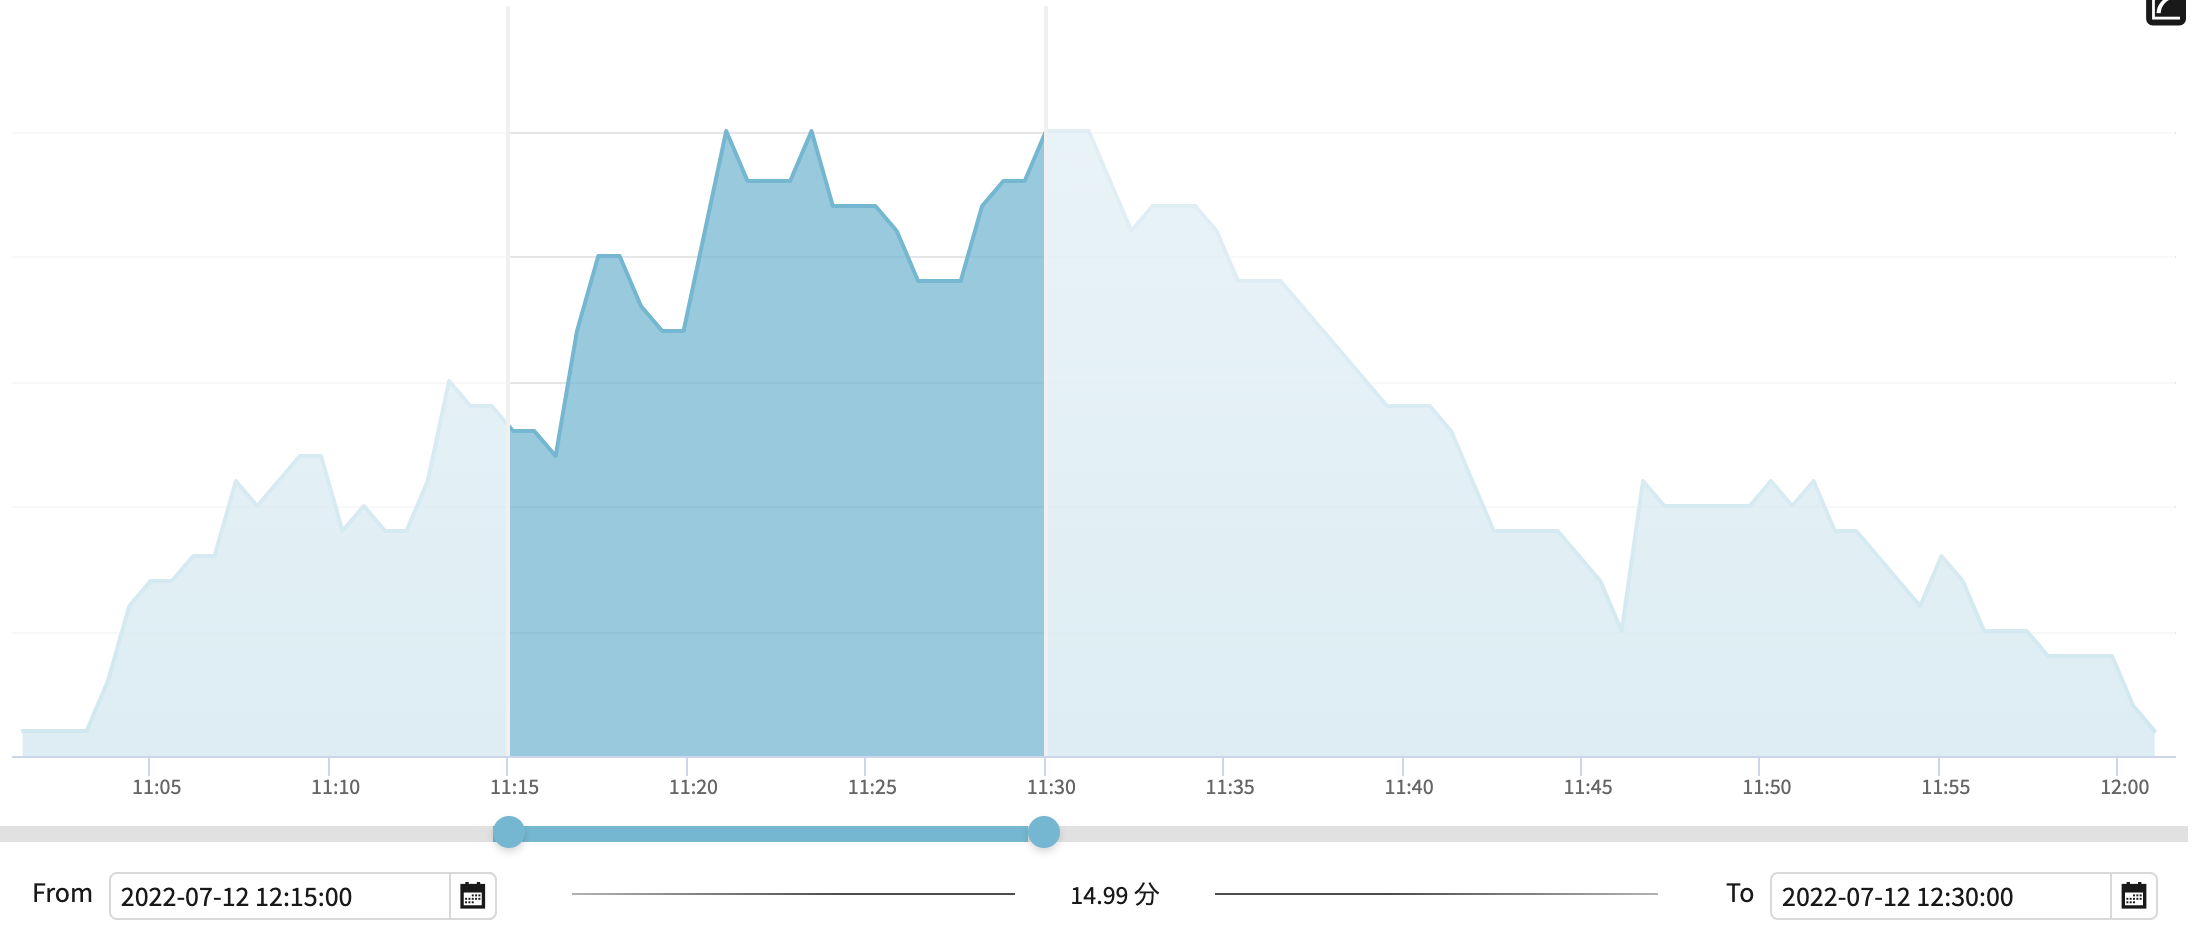
\includegraphics[width=14cm]{712a.png}
  \caption{計測日時:7/12 12:15〜12:30,来店数:43人の時間軸}
  \label{fig:712a}
\end{figure}

\begin{figure}[H]
  \centering
  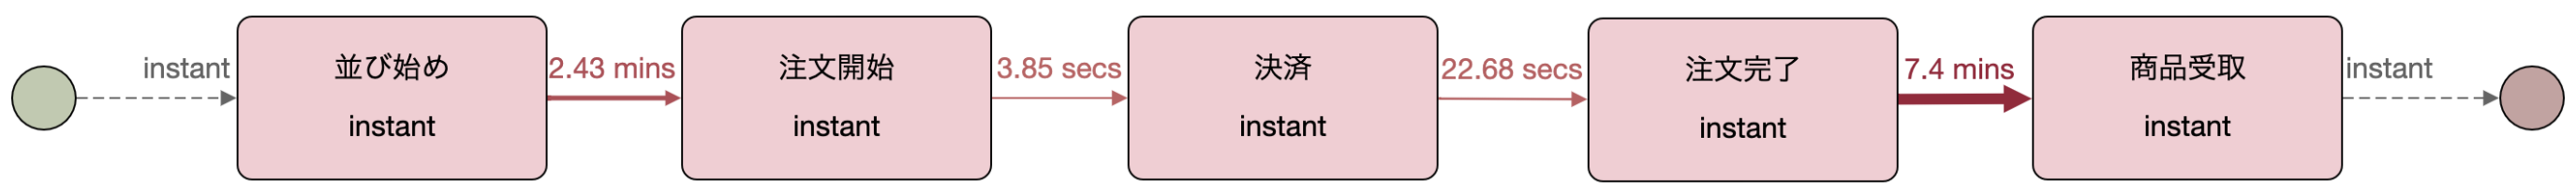
\includegraphics[width=15cm]{712b.png}
  \caption{計測日時:7/12 12:15〜12:30,来店数:43人の各計測項目の平均時間}
  \label{fig:712b}
\end{figure}


\begin{figure}[H]
  \centering
  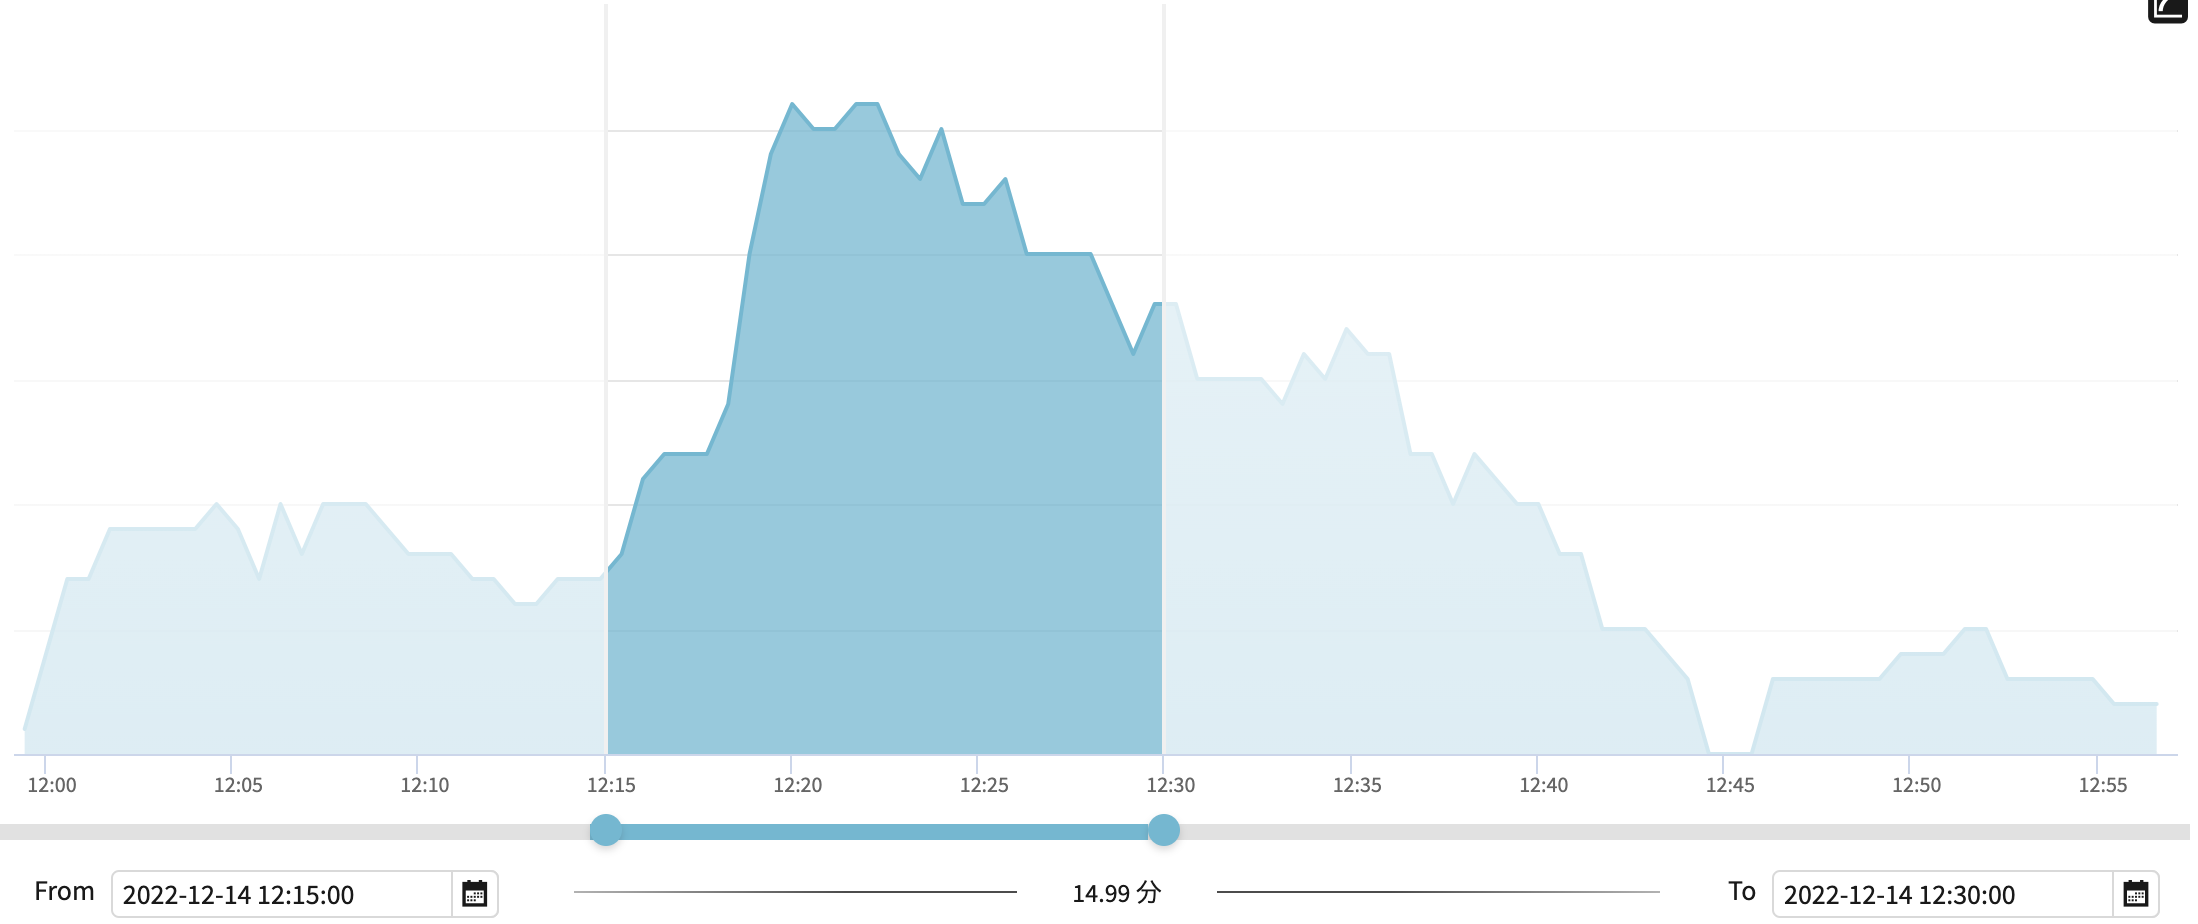
\includegraphics[width=15cm]{1214a.png}
  \caption{計測日時:12/14 12:15〜12:30,来店数:38人の時間軸}
  \label{fig:1214a}
\end{figure}
\begin{figure}[H]
  \centering
  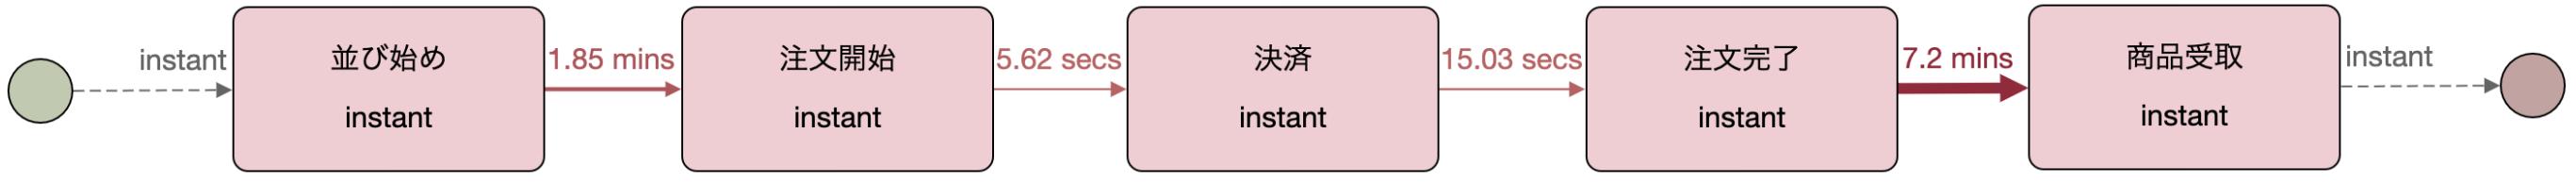
\includegraphics[width=15cm]{1214b.png}
  \caption{計測日時:12/14 12:15〜12:30,来店数:38人の各計測項目の平均時間}
  \label{fig:1214b}
\end{figure}


\begin{figure}[H]
  \centering
  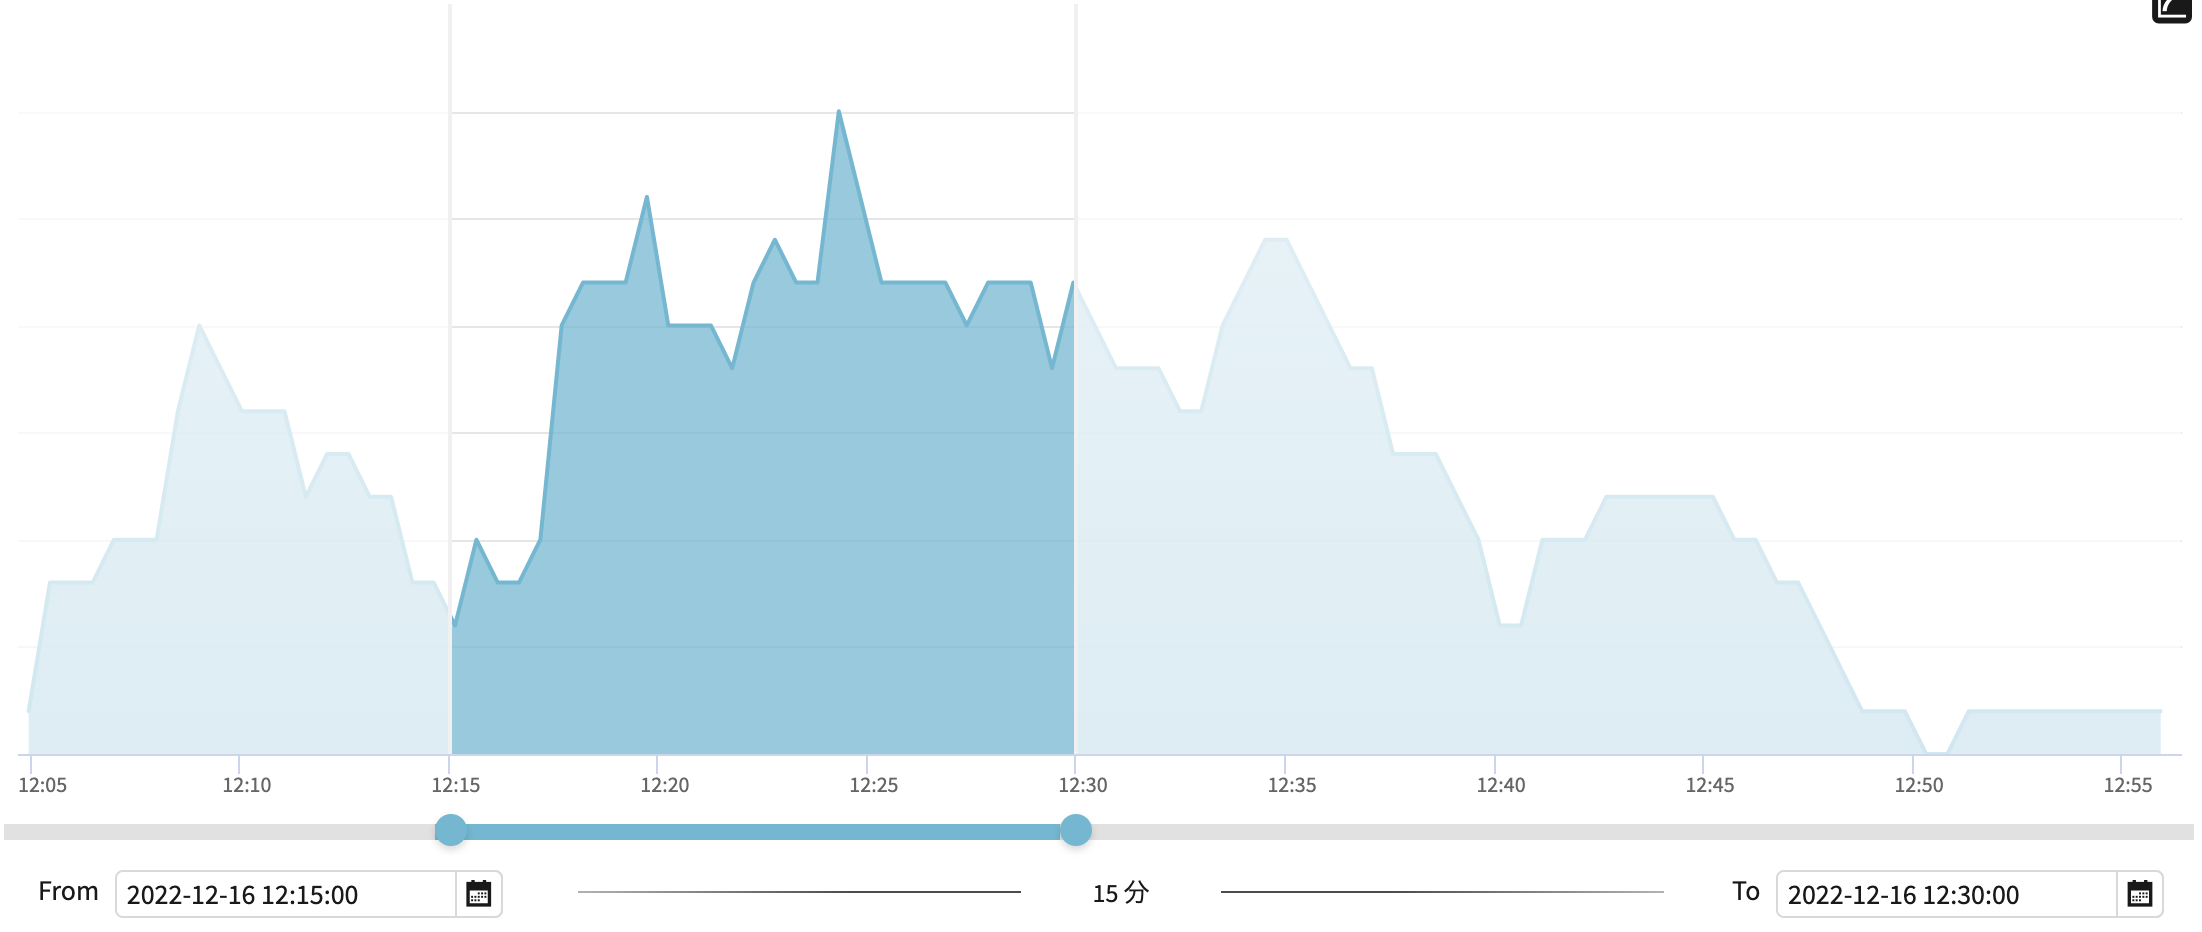
\includegraphics[width=15cm]{1216a.png}
  \caption{計測日時:12/16 12:15〜12:30,来店数:28人の時間軸}
  \label{fig:1216a}
\end{figure}
\begin{figure}[H]
  \centering
  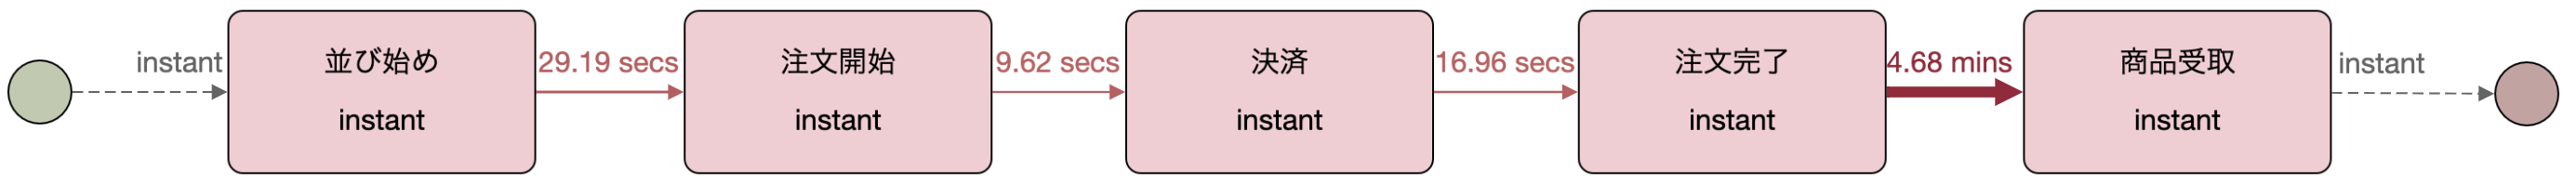
\includegraphics[width=15cm]{1216b.png}
  \caption{計測日時:12/16 12:15〜12:30,来店数:28人の各計測項目の平均時間}
  \label{fig:1216b}
\end{figure}

%------------------------------------------------------------------




\newpage
%------------------------------------------------------------------
5日間の12:00〜13:00と12:15〜12:30における来店数やその割合、
各計測項目の平均時間を表\ref{table6}に示す。

\begin{table}[H]
 \begin{center}
   \caption{}
   \begin{tabular}{|c|c|c||c|c|c|c|} \hline
日時 & 来店数 & 割合 & 行列時間 & 注文時間 & 決済時間 & 商品受取待ち時間 \\ \hline \hline
2022/07/08 12:00〜13:00 & 52 & 100\% & 43秒    & 10秒 & 22秒 & 6分9秒 \\ \hline
2022/07/08 12:15〜12:30 & 37 & 71\%  & 50秒    & 6秒 & 28秒  & 7分3秒 \\ \hline \hline

2022/07/11 12:00〜13:00 & 49 & 100\% & 1分12秒 & 3秒 & 16秒 & 5分43秒 \\ \hline
2022/07/11 12:15〜12:30 & 27 & 55\%  & 1分38秒 & 4秒 & 7秒   & 5分51秒 \\ \hline \hline

2022/07/12 12:00〜13:00 & 75 & 100\% & 2分1秒  & 5秒  & 25秒 & 7分21秒 \\ \hline
2022/07/12 12:15〜12:30 & 47 & 63\%  & 2分26秒 & 4秒 & 27秒  & 7分24秒 \\ \hline \hline

2022/12/14 12:00〜13:00 & 73 & 100\% & 1分10秒 & 6秒 & 14秒 & 6分25秒 \\ \hline
2022/12/14 12:15〜12:30 & 38 & 52\%  & 1分38秒 & 6秒 & 15秒  & 7分32秒 \\ \hline \hline

2022/12/16 12:00〜13:00 & 61 & 100\% & 39秒 & 11秒  & 16秒 & 4分4秒 \\ \hline
2022/12/16 12:15〜12:30 & 28 & 46\%  & 28秒 & 10秒 & 17秒   & 4分34秒 \\ \hline
  \end{tabular}
 \label{table6}
 \end{center}
\end{table}


表\ref{table6}の「割合」より、5日間いずれも12:15〜12:30までの15分の間に、1時間の間に来店する客の半数前後が来店している事から12:15〜12:30までの15分の間は混雑している時間だと伺う事ができる。
行列時間は5日中4日が12:15〜12:30の方が長くなり、
来店数が増加するに連れ行列時間も長くなる傾向にある事が分かる。
注文時間や決済時間は券売機と客の1-1の関係なので来店数によらないものだと考えられる。
商品受取待ち時間も行列時間と同様に5日中5日が12:15〜12:30の方が長くなり、
来店数が増加するに連れ商品受取待ち時間も長くなる傾向にある事が分かる。
%------------------------------------------------------------------


















\newpage

\section{結論・今後の課題}






\newpage

\begin{thebibliography}{99}
\bibitem{bibi1} 宇都宮陽一, 奥田隆史. 多段待ち行列モデルを用いた店舗サービスへの it 導入がもたらす影響の分析. 情報処理学会研究報告, 数理モデル化と問題解決 (MPS), 2017.
\bibitem{bibi2} 小池響. 待ち行列理論を用いた事前注文・事前決済 プラットフォームの開発と評価. 卒業論文、近畿大学理工学部情報学科, 2021.
\bibitem{bibi3} 福永光. 待ち行列理論による受け入れ人数の自動調整機能付き事前注文決済システムの開発と評価. 卒業論文、近畿大学理工学部情報学科, 2022.
\bibitem{bibi4}藤井遼. 事前注文・事前決済プラットフォームの開発と導入による待ち行列の評価-事前注文・事前決済プラットフォームの開発-. 卒業論文、近畿大学理工学部情報学科, 2020.

\bibitem{bibi6}5割以上の飲食店が新型コロナウイルスの影響でテイクアウトを開始/931名に聞いた飲食店の年末の営業と採用活動に関する調査 https://www.foods-ch.com/news/prt\_76113/  
\bibitem{bibi7}消費者に定着しつつある飲食店のテイクアウト・デリバリーサービス\\
https://www.jfc.go.jp/n/findings/pdf/seikatsu20\_1215a.pdf
\bibitem{bibi8}豊泉洋 (早稲田大学会計研究科教授):スタバの並び方って変じゃない?:順番待ちの数学,YOMIURI ONLINE, 入手先 http://www.yomiuri.co.jp/adv/wol/opinion/science150105.html
\bibitem{bibi9}オープンソースではじめるプロセスマイニング. ハートコア株式会社,2022
\end{thebibliography}
\end{document}
